\section{Results}
\label{sec:results}

\subsection{Reserve economics and backup service}

Figure~\ref{fig:frontier} and Table~\ref{tab:frontier} report the Houston 2024 validation replay. A fixed 20\% reserve serves the first five hours of \FixedPromise\ of simulated episodes. The hazard-threshold rule with $\varepsilon=0.1$ yields \ThresholdPromise, with an annualized margin difference of \$\ThresholdDelta\ per home and paired 95\% interval $[\ThresholdLow,\ThresholdHigh]$. Its annualized unserved energy is \ThresholdUnserved\ kWh per home, compared with \FixedUnserved\ for fixed 20\%. Promise fulfillment and total unserved energy measure different parts of service: a controller can protect a short commitment while still exhausting its battery during a longer interruption.

The observed promise increase is \ThresholdPromiseDelta\ percentage points. Its paired window-bootstrap interval is $[\ThresholdPromiseDeltaLow,\ThresholdPromiseDeltaHigh]$ points and includes zero. Thus the simulated economic gain has a positive paired interval, while the service improvement is sensitive to which recorded storm windows appear in a resample. Neither interval establishes a future household reliability guarantee.

Tables~\ref{tab:tails}, \ref{tab:households}, and \ref{tab:seasonal} give cash tails, household outcomes, and seasonal window cohorts. The seasonal grouping retains each complete replay window and states how boundary-crossing windows are assigned; it does not change the full-year comparison or selection criterion.

\begin{figure}[t]
  \centering
  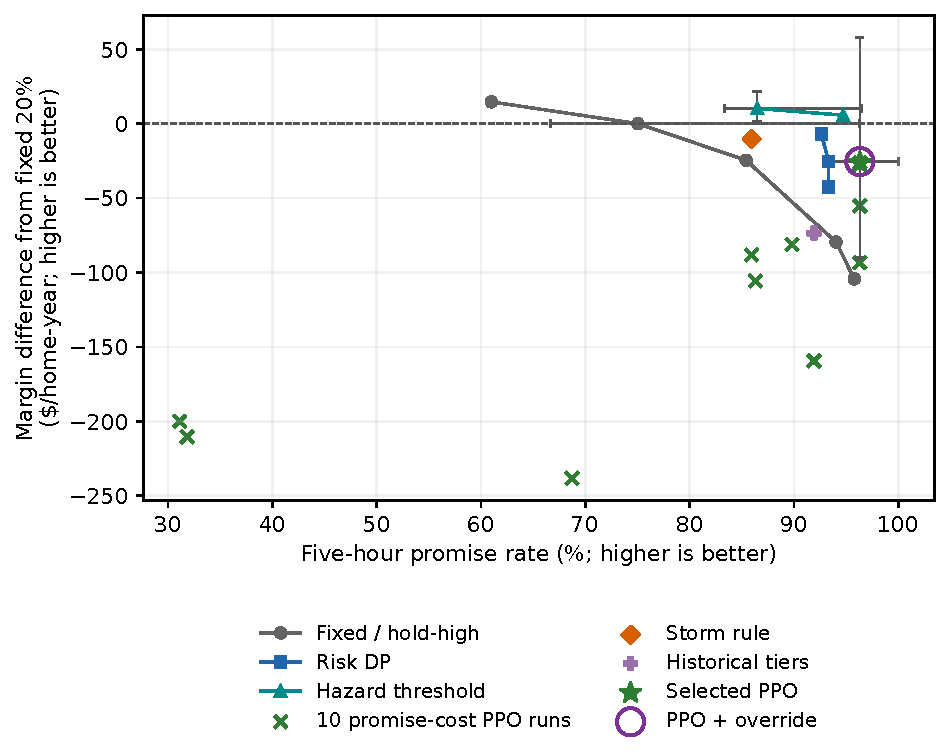
\includegraphics[width=\linewidth]{figs/frontier.pdf}
  \caption{Houston 2024: economics versus simulated backup service. Higher values on either axis are preferable. Margin is paired against fixed 20\% and adjusted for terminal inventory. Crosses show every promise-cost PPO candidate; the selected candidate and its alert override are marked separately. Error bars for fixed 20\%, threshold 0.1, and guarded PPO show 95\% window-bootstrap intervals. Lines connect settings within a family and do not imply a fitted Pareto frontier.}
  \label{fig:frontier}
\end{figure}

\begin{table}[t]
  \centering\small
  \begin{tabular}{lrrr}
\toprule
Controller & $\Delta$ margin [95\% CI] & Promise [95\% CI] & Unserved \\
\midrule
Fixed 20\% & +0.0 [0.0, 0.0] & 75.0 [66.7, 96.3] & 204.0 \\
Fixed 50\% & -79.5 [-138.5, -34.1] & 94.0 [92.0, 100.0] & 189.1 \\
Hold near 90\% & -104.3 [-145.1, -72.6] & 95.8 [93.5, 100.0] & 177.8 \\
Storm rule & -10.2 [-17.6, -3.7] & 85.9 [83.3, 97.9] & 190.1 \\
Historical tiers & -73.6 [-126.4, -32.4] & 91.9 [90.3, 100.0] & 189.9 \\
Risk DP 5 & -25.4 [-37.7, -15.2] & 93.3 [87.0, 100.0] & 191.8 \\
Threshold 0.1 & +10.2 [1.7, 21.7] & 86.5 [83.4, 96.5] & 195.2 \\
Selected PPO & -26.1 [-91.2, 57.9] & 96.3 [93.5, 100.0] & 172.7 \\
PPO + override & -25.5 [-90.3, 58.1] & 96.3 [93.5, 100.0] & 172.7 \\
\bottomrule
\end{tabular}

  \caption{Houston 2024, 100 simulated homes. Margin difference is USD/home-year and unserved energy is kWh/home-year; promise is a percentage. Brackets are 95\% bootstrap intervals. Higher margin/promise and lower unserved energy are preferable. All regular windows, including the final partial window, receive duration-appropriate weight. Named event evaluations are excluded from these aggregates.}
  \label{tab:frontier}
\end{table}

The risk-priced dynamic program at $\lambda_r=5$ yields \RiskPromise\ promise and a \$\RiskDelta\ margin difference from fixed 20\%. This comparison exposes the cost of preserving energy under its surrogate risk charge. The released summary also includes all fixed floors, the high-SOC preference, historical tiers, both risk thresholds, and the oracle-onset timing reference. A difference between forecast and oracle-onset variants reflects this particular surrogate's response to changed inputs; it is not an identified fraction of the value of perfect information. The market-lookahead reference additionally changes price and load information, so it is reported separately.

\subsection{Learning, seed dispersion, and transfer}

The validation criterion selects \SelectedRun\ from ten promise-cost candidates. Its promise rate is \LearnedPromise\ and its margin difference is \$\LearnedDelta\ per home-year. Across those ten runs, promise spans \PromiseSeedLow--\PromiseSeedHigh\ and median margin difference is \$\PromiseSeedMedianDelta. Of these \PromiseCandidateCount\ runs, \PromiseBelowFixedCount\ have lower promise than fixed 20\%, and \PromiseNegativeMarginCount\ have lower inventory-adjusted margin. Table~\ref{tab:promise-seeds} reports every candidate, and Table~\ref{tab:other-seeds} reports all eleven full-cost and reserve-ablation runs. Mean SOC and throughput help distinguish retaining charge from actively timing market opportunities; a single selected point cannot describe training stability.

\begin{figure}[tbp]
  \centering
  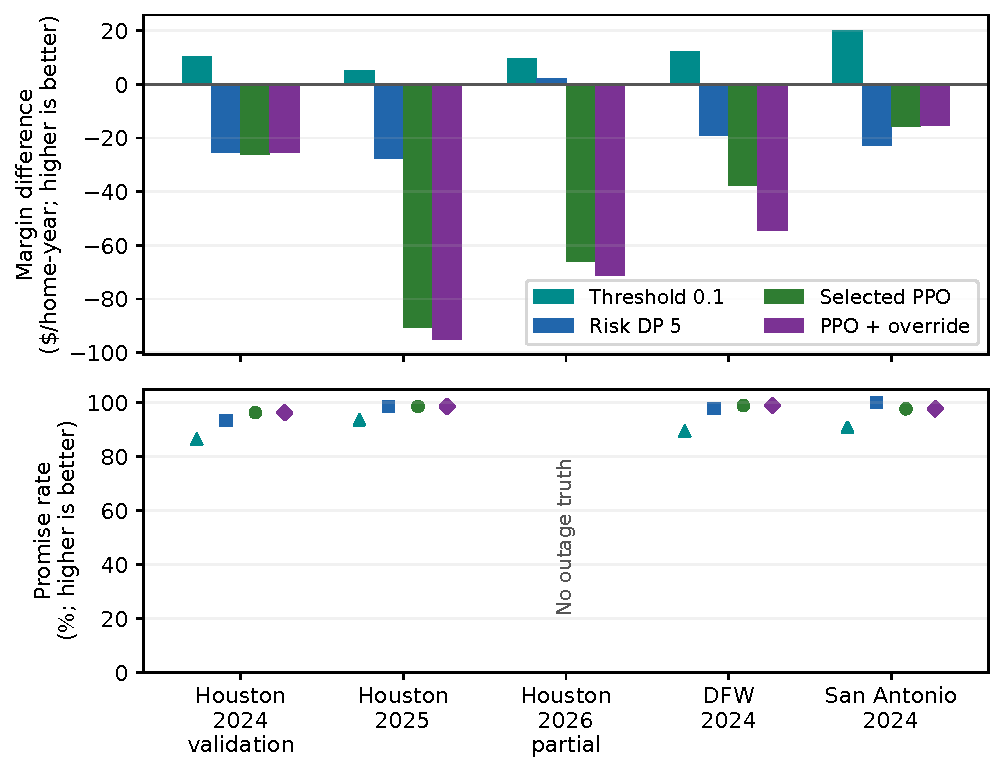
\includegraphics[width=\linewidth]{figs/transfer.pdf}
  \caption{Transfer of the fixed validation choices. The upper panel shows annualized margin differences from the local fixed-20\% reference; positive is preferable. The lower panel shows episode-pooled five-hour promise; higher is preferable. The 2026 replay is partial-year and has no observed outage truth. Metro comparisons use the same tariff and hardware assumptions with different public building pools and county traces.}
  \label{fig:transfer}
\end{figure}

On Houston 2025, threshold 0.1 differs from fixed 20\% by \$\TestThresholdDelta\ per home-year, and the selected learned policy by \$\TestLearnedDelta; their promise rates are \TestThresholdPromise\ and \TestLearnedPromise. On available 2026 prices, the corresponding margin differences are \$\PartialThresholdDelta\ and \$\PartialLearnedDelta. These chronological tests assess reuse of the frozen controller. They do not retune a policy for the new year or infer the causal effect of a market redesign. Geographic outcomes appear in Figure~\ref{fig:transfer} and the complete released summary.

The validation improvement therefore does not uniformly transfer as a gain on both axes. In 2025, threshold 0.1 has higher modeled margin but lower promise than fixed 20\% (\TestFixedPromise). The market-only 2026 comparison cannot resolve that service tradeoff.

The threshold's 2024 metro outcomes also differ. In DFW it yields \DFWThresholdPromise\ promise versus \DFWFixedPromise\ for fixed 20\%, with a \$\DFWThresholdDelta\ margin difference per home-year. In San Antonio the corresponding values are \SanAntonioThresholdPromise\ versus \SanAntonioFixedPromise\ and \$\SanAntonioThresholdDelta. These comparisons pool \DFWEpisodes\ and \SanAntonioEpisodes\ simulated household episodes, respectively, with outcomes correlated through shared county traces.

Six pre-specified windows also test fleets of 100, 500, and 1,000 homes, a 70\% Core mix, and 20\% communication dropout (Table~\ref{tab:structure}). All five scenarios retain the same six windows and include fixed, storm, risk-DP, learned, and guarded learned controls. Those results describe sensitivity within the simulated pool. Resampling a larger fleet does not create new measured homes or establish asymptotic reliability. Table~\ref{tab:latency} reports complete CPU decision/simulation wall time under a stated backend; it is not a field communication-latency measurement.

\subsection{Storms, warning coverage, and the charging override}

Uri's scored intervals are held out of PPO training; it is an event holdout rather than a chronological backtest (Appendix~\ref{app:repro}). On its Houston window, selected PPO has promise \UriLearnedPromise\ and margin \$\UriLearnedMargin\ per home-week. Adding the alert override changes these values to \UriGuardedPromise\ and \$\UriGuardedMargin. Fixed 20\% and risk DP 5 yield \UriFixedPromise\ and \UriRiskPromise. Figure~\ref{fig:traces} shows energy and unserved-demand trajectories; Table~\ref{tab:events} also reports Elliott, derecho, Beryl, and a DFW Elliott replay. A zero-episode window has no reliability score. These lower-severity cases and the synthetic tests extend the audit beyond one extreme storm.

The warning system limits any interpretation of Proposition~\ref{prop:charging}. Across all six evaluated counties in 2019--2025, \MassEvents\ county episodes reach 5\% customers out. A qualifying alert is active at onset in \AlertCoverage, but continuous lead is at least four hours in only \AlertLeadCoverage\ (Table~\ref{tab:alerts}). Four hours is the conservative minimum-to-90\% charging time across all three hardware presets. Alert presence sometime during the preceding day is reported separately and is not substituted for an active, sustained warning. This audit uses county episodes merged across gaps of up to four hours, distinct from the one-hour household flicker merge in promise scoring.

\begin{figure}[tbp]
  \centering
  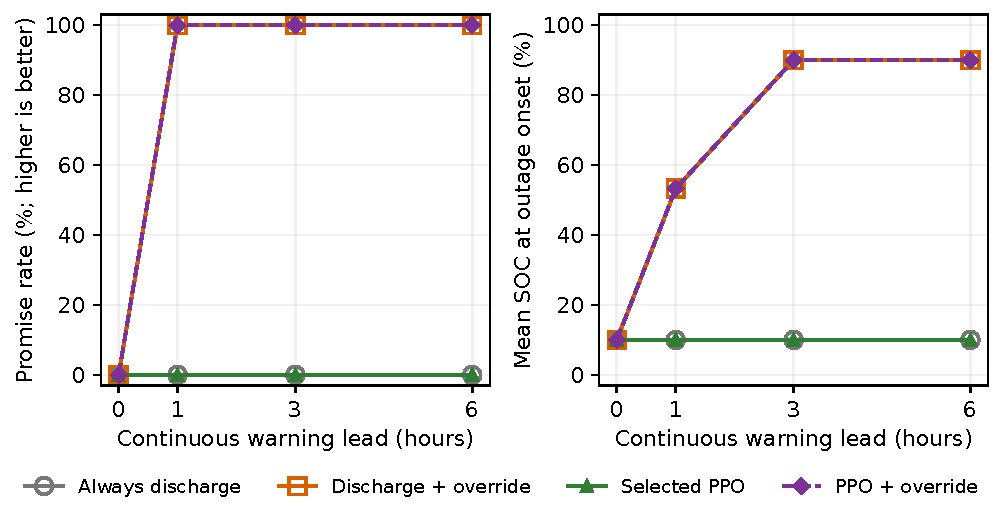
\includegraphics[width=\linewidth]{figs/stress.pdf}
  \caption{Controlled joint-event stress: \$5,000/MWh price, eight-hour outage, 10\% initial SOC, 25 kWh batteries, 2 kW demand, no PV/dropout, and full state of health. Warning lead varies while other inputs remain fixed. Promise rate is higher-is-better; onset SOC explains the available backup energy. The wider synthetic suite includes 86 indexed cases, including false/missed alerts, load uplift, reduced state of health, and dropout.}
  \label{fig:stress}
\end{figure}

The synthetic suite evaluates an always-discharge proposal and the selected PPO, each with and without the override. Every one of \SufficientTests\ guarded comparisons meeting the nominal sufficient-condition subset serves the five-hour promise. This verifies the implementation for those cases rather than extending the proposition to cases outside its premises. Short or missing warnings and unavailable charging require separate outcomes, which remain in the released results. False alerts can cost up to \$\FalseAlertWorstCost\ per home over a complete 48-hour synthetic episode. Their paired cash-margin differences after the warning ends reach \$\FalseAlertAfterDifference\ in magnitude. Consequently, charging cost cannot be assessed solely during alert hours.

\FloatBarrier
\section{Distribution and battery-life consequences}
\label{sec:system}

\paragraph{Static AC audit.}
Dispatch affects household net exchange even though market prices are exogenous. We replay three days on one SMART-DS Austin feeder~\citep{smartds}, randomly attach batteries at 30\% or 100\% of load locations, and compare with identical load/PV profiles and no battery dispatch. This is an illustrative placement study using Houston profiles on a synthetic Austin topology, not a calibrated network representation of those homes. Grid exchange is zero while a simulated home is islanded. The original feeder load models are retained, with reactive demand set to 0.33 times positive real demand.

Table~\ref{tab:ac} reports convergence, voltage ranges, and the fraction of intervals with voltage or line-rating violations. The aggregate solver-convergence rate is \ACConvergence. Under the stated reporting rule, the reference already exhibits undervoltage, overvoltage, and line overloads; 30\% penetration cannot be described as uniformly benign. We retain every phase-node voltage at buses reachable in the bus-level source graph, including near-zero values, rather than filtering by an acceptable-voltage band. Eighteen phase nodes at unreachable buses are reported separately. Bus-level reachability does not certify phase energization. Snapshot convergence alone is not proof of acceptable operation, protection coordination, or dynamic stability.

\paragraph{Aging-model sensitivity.}
Table~\ref{tab:aging} compares four windows and 20 homes per window. A throughput model predicts \FixedETFade\ annualized fade for fixed 20\% and \HoldETFade\ for the hold-high preference. Under the SOC/temperature-dependent BLAST model, repeating those windows predicts \FixedBLASTFade\ and \HoldBLASTFade, respectively. These comparisons expose different penalties for cycling and high SOC. They do not measure the lifetime of the specified commercial packs. The throughput coefficient uses a complete charge/discharge cycle as its normalization; the corrected release records the factor-of-two reporting correction to earlier outputs. The linear-calendar, throughput, and rainflow coefficients and the BLAST chemistry/repetition convention are specified in Appendix~\ref{app:aging}. Dispatch is held fixed across aging models and receives no aging charge in the main comparison.
